\documentclass{article}
\usepackage[utf8]{inputenc}
\usepackage{float}
\usepackage{xcolor}
\usepackage{graphicx}
\usepackage{amsmath}
\usepackage{amssymb}

\usepackage{hyperref}
\hypersetup{
    colorlinks=true,
    linkcolor=blue,
    filecolor=magenta,      
    urlcolor=blue,
}

\title{Scientific Computing - Molecular dynamics \\ Group F}
\newcommand{\subtitle}{Problem sheet 2}
\author{
    Jimin Kim \\
    Christian Nix \\
    Noah Schlenker
}
\date{\today}

\begin{document}

\maketitle

\begin{center}
    \LARGE \subtitle{}
\end{center}

\section{Pull request}
\label{sec:pr}
The pull request can be found \href{https://github.com/noahpy/MolSim-SS24/pull/20}{here}.

\section{Unit Tests}
\label{sec:ut}

\begin{itemize}
    \item We already successfully implemented \verb|gtest| in the previous assignment, providing a robust foundation for subsequent testing enhancements.
    \item Integration of \verb|gtest| through CMake is managed within its dedicated CMake module, reinforcing a decentralized and modular system architecture.
    \item cmake verifies the presence of \verb|gtest| before attempting to fetch the library via CMake.
    \item To avoid building the same source files twice (once for MolSim and once for tests), the project source files are added as a library, then statically linked to the tests target.
    \item Building upon the tests included in the previous assignment, the additions for this iteration encompass tests for the force calculation via the Lennard-Jones potential and the particle generator functionality.
    \item The tests for the Lennard-Jones force calculation perform direct verification of computational correctness (see \texttt{tests/physics/testForceLJ.cpp}).
    \item Tests for the particle generator validate the structural integrity of generated cuboids and the properties of contained particles \newline(see \texttt{tests/simulation/testParticleGenerator.cpp}).
    \item Further tests for new input and output systems were also included (see \texttt{tests/io})
\end{itemize}

\section{Realization of Continuous Integration}
\label{sec:ci}

\begin{itemize}
    \item We implemented CI through Docker, ensuring a consistent and isolated environment for all integration and testing processes.
    \item We utilized `nektos/act`, a tool that simulates GitHub Actions locally, allowing us to validate workflows before pushing to the repository.
    \item The CI pipeline was expanded to include dynamic analysis with the GCC `-fsanitize=address` flag and integrated unit tests within the CI pipeline to verify that all tests pass before any code merges into the master or \verb|assignment*| branches, enhancing code reliability.
    \item Branch protection rules were successfully configured for the \verb|master| and all \verb|assignment*| branches, ensuring no direct pushes can occur and all merges require successful CI checks and pull-request reviews from at least one other team mate.
    \item This allows our team to be aware of any and all modifications made by other teammates, which will become an issue once the code base grows and keeping track becomes more difficult
\end{itemize}

\section{Logging Configuration via spdlog}
\label{sec:spd}

\begin{itemize}
    \item In alignment with our methodology for integrating \verb|gtest|, \verb|spdlog| was incorporated using a CMake module, including a pre-fetch check to ensure its availability before fetching it via CMake.
    \item We opted to utilize the functions provided by \verb|spdlog|, favoring their type safety, which aids in more explicit and clear code management and debugging. This approach ensures that each logging call is checked at runtime.
    \item Although \verb|spdlog| macros offer potential performance enhancements by omitting logging code at compile-time for disabled log levels, we determined that this advantage was not critical for our current project scope, as it utilizes run-time configuration of the global log level.
    \item For us, the slight performance gain from the lazy evaluation of macro arguments (where evaluation occurs only if the level check passes) did not outweigh the benefits of using functions. However, we may reconsider this decision in future assignments if a significant performance difference is observed.
    \item The logging level can be dynamically adjusted via the command-line option \texttt{-l}, facilitating the ease of toggling between different logging levels according to the needs of runtime diagnostics.
\end{itemize}

\section{Adjustment of program frame}
\label{sec:adj}
We additionally extended on our project structure with a few classes. 
No fundamental changes were necessary, so we would evaluate our project structure from the last assignment as a success. The following UML shows the relevant changes:
\begin{figure}[H]
    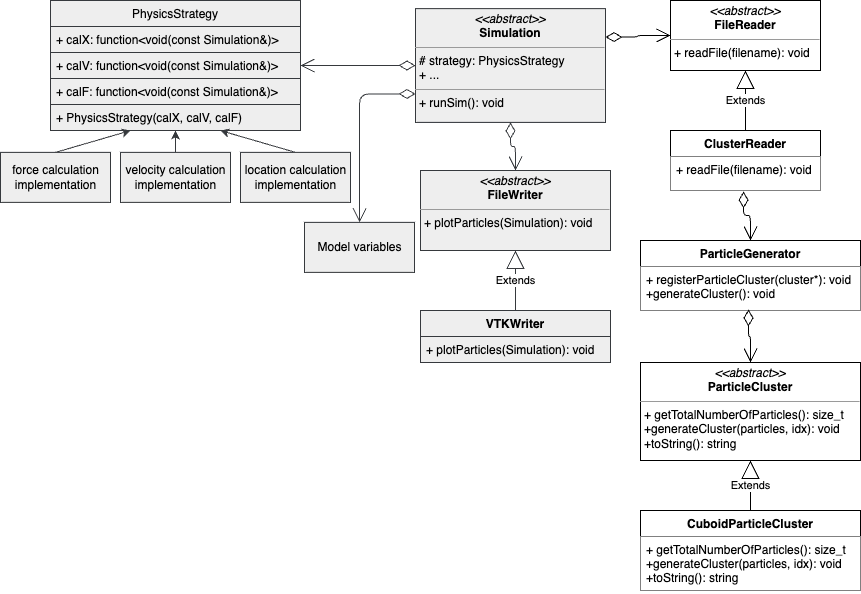
\includegraphics[width=\textwidth]{/home/jimin/MolSim2/docs/res/UML}
    \caption{UML-like diagram showing our modelling ideas relevant to the assignment. Note that only the white classes are new or modified; the grey classes are unchanged.}
\end{figure}


\subsection{I/O Expansion}
\label{subsec:file}

\begin{itemize}
    \item We have enhanced our I/O functionalities to support various input file formats.
    \item Introduction of specialized file-reader functions enabled us to handle different file formats, including cluster and ASCII art data (more on this in the last section). These functions extend the capabilities of the base reader function (see \texttt{src/io/fileReader}).
\end{itemize}

\subsection{Simulation Expansion}
\label{subsec:sim}

\begin{itemize}
    \item The simulation for using the Lennard-Jones-potential was included (\verb|src/simulation|).
    \item For calculating the forces derived from the Lennard-Jones-potential, we rearranged the formula provided on the problem sheet, to avoid unnecessary calculations
    \begin{align}
        F_{i,j} &= -\frac{\epsilon \cdot 24}{(||x_i-x_j||_2)^2} \left( \left( \frac{\sigma}{||x_i-x_j||_2} \right) ^6 - 2 \left( \frac{\sigma}{||x_i-x_j||_2} \right) ^{12} \right) (x_i-x_j) \\
                &= \frac{-\epsilon \cdot 24}{(||x_i-x_j||_2)^2} \left(  \frac{\sigma ^6 }{||x_i-x_j||_2 ^6 } + \frac{-2 \cdot \sigma^{12}}{||x_i-x_j||_2^{12}}  \right) (x_i-x_j)
    \end{align}
    Where  $-\epsilon \cdot 24 =: \alpha$, $\sigma ^6 =: \beta$, and $-2 \cdot \sigma^{12} =: \gamma$ are constant for a simulation of only one type of particle. We therefore only calculate these once upon initialization of the Lennard-Jones-Simulation, as judging from the presentation of week one, we will only be dealing with particles of one type, where $\sigma$ and $\epsilon$ are true for all particles in the simulation. \\
    Further, let $x_i-x_j =: \delta \in \mathbb{R}^3$
    \begin{align}
        F_{i,j} &= \frac{\alpha}{(||\delta||_2)^2} \left(  \frac{\beta}{||\delta||_2 ^6 } + \frac{\gamma}{||\delta||_2^{12}}  \right) \cdot \delta \\
        &= \frac{\alpha}{\delta ^T\delta} \left(  \frac{\beta}{(\delta ^T\delta) ^3} + \frac{\gamma}{(\delta ^T\delta) ^6}  \right) \cdot \delta \\
        &= \frac{\alpha}{\delta ^T\delta} \left(  \frac{\beta}{(\delta ^T\delta) ^3} + \frac{\gamma}{((\delta ^T\delta) ^3) ^2}  \right) \cdot \delta
    \end{align} 
    \item We included a factory function for the simulations that allows for interchangeable scenarios i.e. to choose between the different simulations we have and will implement.
\end{itemize}

\subsection{Additional Arguments for the Program}
\label{subsec:arg}

\begin{itemize}
    \item We have included several additional command-line options (\verb|src/io/argparse|). These options aim to give the user full control and flexibilty over which simulation and which input he wants to combine.
    \item The parameters \texttt{epsilon} and \texttt{sigma} can now be specified via command-line if the default values are not suitable for the user's needs.
    \item Additional command-line arguments have been introduced to allow users to specify the input file format, supporting both clusters and ASCII art (options \texttt{-c} or \texttt{-a}).
    \item Users now have the flexibility to set the simulation type with \texttt{-s} and the file-writer type with \texttt{-w} enhancing runtime configurability.
    \item This flexibility ensures that we will always stay "backwards compatible", meaning we can run every simulation we were assigned before :)
    \item To deal with this flexibility of different child classes we implemented factory functions, which return a pointer to the correct class depending on user input.
\end{itemize}

\subsection{Particle Generator}
\label{subsec:particleGenerator}

\begin{itemize}
    \item The \verb|ParticleGenerator| class has two methods to generate clusters of particles (in \verb|src/models/generators|)
    \begin{enumerate}
        \item \verb|registerCluster|: This method takes a unique pointer to a \verb|ParticleCluster| object and pushes it onto a vector of pointers to store the references for the following generation of the particles
        \item \verb|generateClusters|: This method will create a vector of the length of all particles in all registered particles and will then call \verb|generateCluster| on every registered \verb|ParticleCluster|
    \end{enumerate}
    \item The advantage of having a dedicated register method is that the number of particles to be generated is known; which allows to allocate a vector of the fitting length at once, instead of adjusting the vector size cluster by cluster or worse, particle by particle
    \item \verb|ParticleCluster| is an abstract class requiring child classes to implement three methods. (i) \verb|getTotalNumberOfParticles| $\rightarrow$ Returns the number of particles in the cluster (ii) \verb|generateCluster| $\rightarrow$ insert all particles into the passed particles vector (iii) \verb|toString| $\rightarrow$ Stringify for logging
    \item We implemented a child class \verb|CuboidParticleCluster| which will generate a cluster as described on the problem sheet.
    \item We decided the \verb|ParticleCluster| to be abstract, so that we can easily add new types of clusters. Looking at the tasks for the next weeks "falling drop" sounded to us, as if we would need to generate spherical clusters in the upcoming weeks
\end{itemize}



\section{Performance testing}
\label{sec:perf}
\begin{itemize}
    \item Benchmarking of the Lennard-Jones calculations on cuboid particle clusters was implemented in its separate folder called \texttt{bench}.
    \item We relied on the \verb|google benchmark| library, which is similar to the \verb|google test| library. This library gets fetched and built if BUILD\_BENCH cmake-option is turned on and no global installation is found.
    \item We already included time measurements in the last assignment, using singular force calculations for pairs of particles. The speedup observed was ca. 1.2 compared to a naive implementation of the force (see \texttt{docs/report/report1}).
    \item The measurements for this assignment are for showcasing the functionality of the new benchmark environment and for comparison to results of other groups with similar hardware specifications.
\end{itemize}
    We ran the simulation the given parameters from the worksheet, without logs and vtk outputs and only measured the computing code part. As a result, the benchmark terminated at around 1min and 44 seconds (104s), as seen in the screenshot below. 

    \begin{figure}[H]
        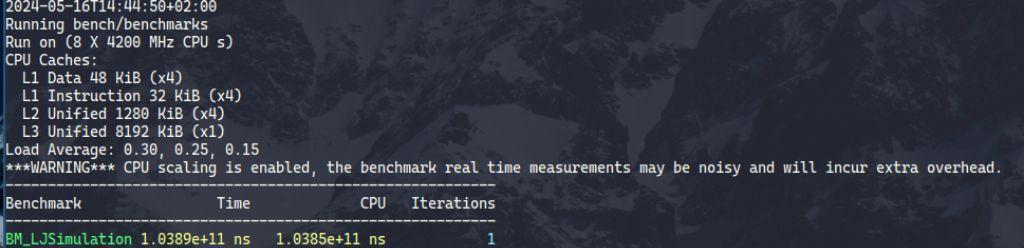
\includegraphics[width=\textwidth]{/home/jimin/MolSim2/docs/res/bench}
        \caption{Output of google benchmark}
    \end{figure}

    The Hardware specs can be observed in the following screenshot (I use arch btw):
    \begin{figure}[H]
        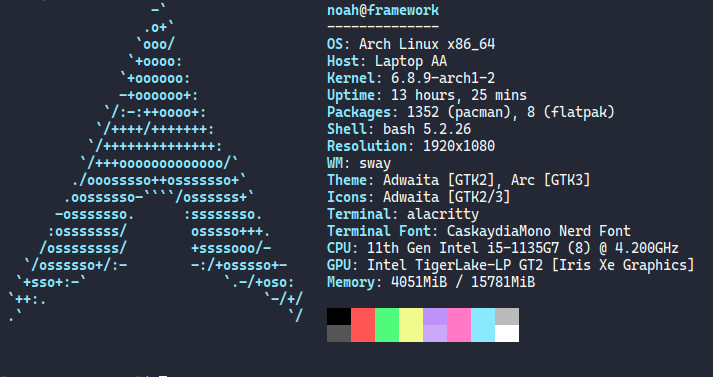
\includegraphics[width=\textwidth]{/home/jimin/MolSim2/docs/res/neofetch}
        \caption{Hardware specs of the benchmark, sorry for the unneseccary joke}
    \end{figure}
   

\section{Miscellaneous}
Everything from here on was not required by the assignment, but we did as we may have seen the necessity or just for fun :)
\subsection{Man page}

\begin{itemize}
    \item We included a man page, which can be accessed by executing the command \texttt{man ./molsim.1} from the root directory of the project.
    \item It includes more specified details for the input formats and the functionalities of our program, as a help message alone could not contain all the details.
\end{itemize}

\subsection{Documentation Hosting}
We now host our doxygen documentation \href{https://noahpy.github.io/MolSim-SS24/}{here} using GitHub pages. 

\subsection{ASCII Art to particles!}
\begin{itemize}
    \item We thought it would be fun to visualize any kind of shapes as a cluster and then let them clash into each other.
    \item As CuboidParticles seemed to be somewhat unflexible, we decided to implement a ASCII art reader (\verb|src/io/fileReader/asciiReader.cpp|), which converts multiple ASCII arts into particle clusters!
    \item So here are picture from two TUM-Logos crashing into each other using Lennard-Jones Simulation (kaboom!). You can also run this by yourself with: \verb|src/Molsim ../input/tum.txt -a -s 1 -e 5 -d 0.0002|
\end{itemize}
\begin{figure}[H]
        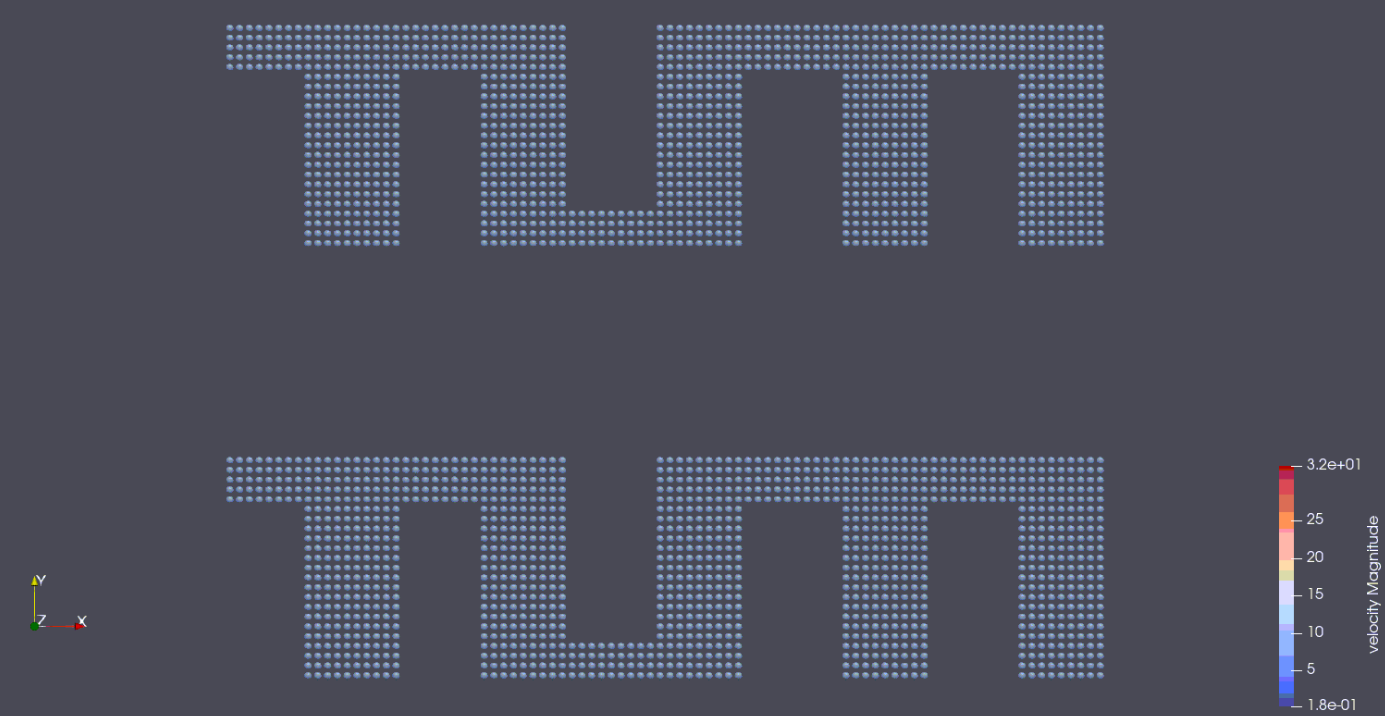
\includegraphics[width=\textwidth]{/home/jimin/MolSim2/docs/res/tum1}
    \end{figure}
\begin{figure}[H]
        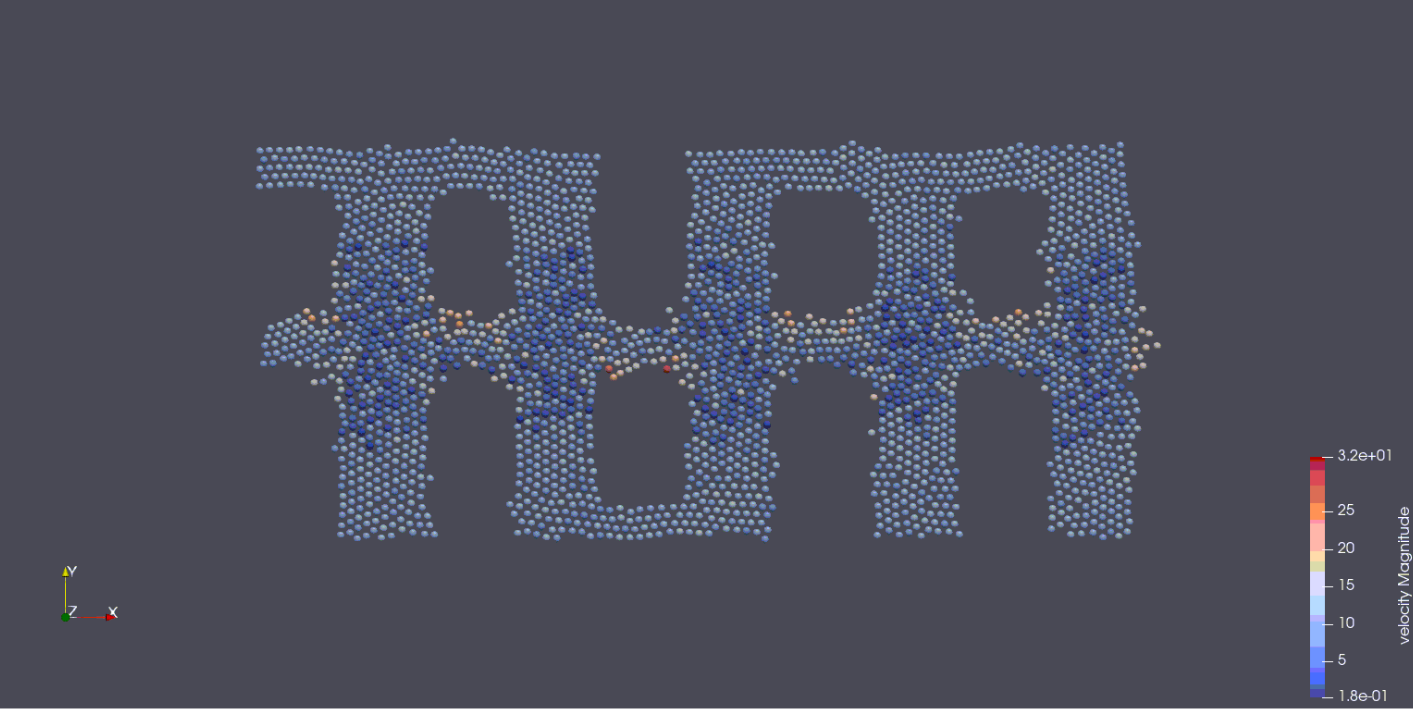
\includegraphics[width=\textwidth]{/home/jimin/MolSim2/docs/res/tum2}
    \end{figure}
\begin{figure}[H]
        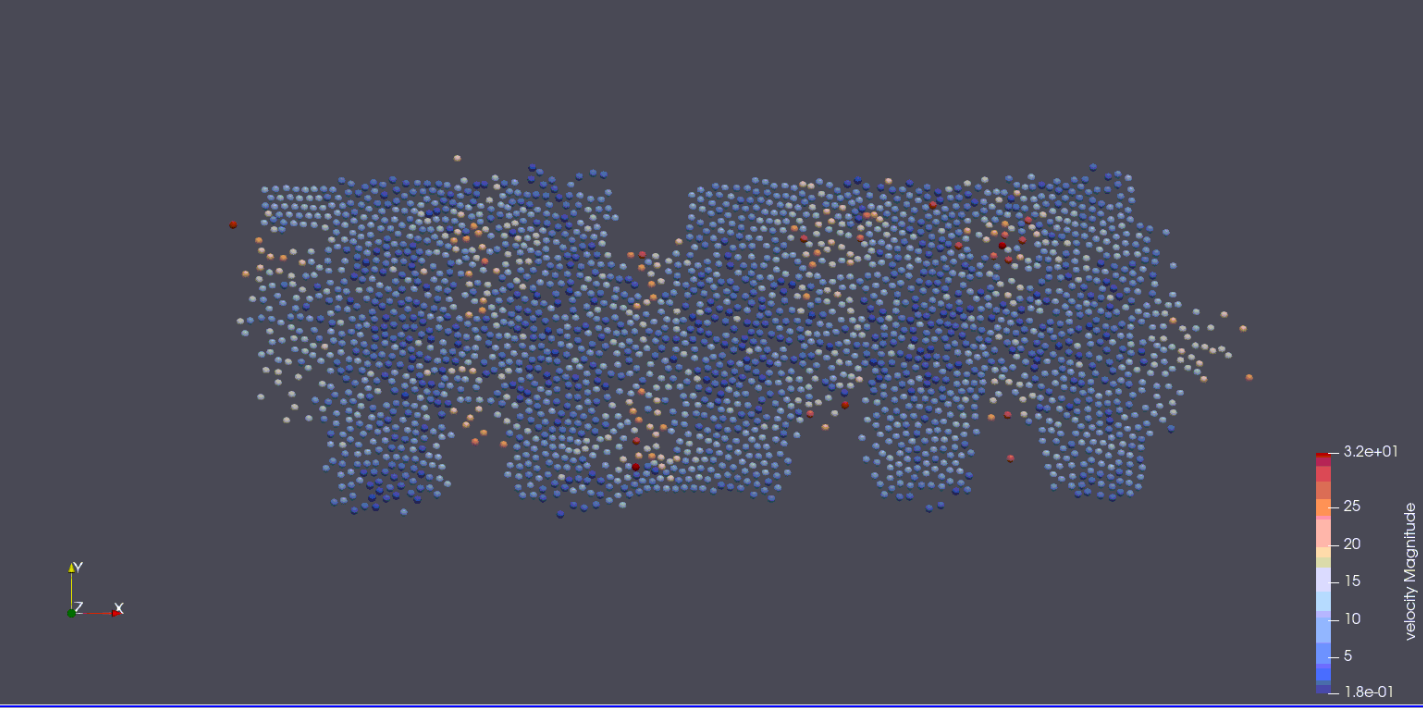
\includegraphics[width=\textwidth]{/home/jimin/MolSim2/docs/res/tum3}
    \end{figure}
\end{document}
